% =====================================================================
%  MẪU BÁO CÁO TIỂU LUẬN HỌC PHẦN HỌC MÁY - Nguyễn Tuấn Anh
%  ---------------------------------------------------------------------
%  Biên dịch bằng XeLaTeX (hoặc LuaLaTeX), chạy 2 lần để cập nhật mục lục.
%  Trên Overleaf: Menu > Compiler > XeLaTeX.
%  Trên máy:      latexmk -xelatex main.tex
%
%  Cách dùng mẫu:
%   1. Sửa THÔNG TIN BÁO CÁO ở mục (A) bên dưới.
%   2. Viết nội dung vào các chương; xóa các đoạn \huongdan{...} khi hoàn thành.
%   3. Đặt hình vào thư mục images/ và thay các khung \khunghinh{...}
%      bằng \includegraphics[width=...]{ten_hinh.png}.
% =====================================================================
\documentclass[12pt,a4paper,oneside]{report}

% Cỡ chữ thân bài 13pt (theo quy định trình bày của bộ môn)
\makeatletter
\renewcommand\normalsize{%
  \@setfontsize\normalsize{13pt}{15.6pt}%
  \abovedisplayskip 12pt plus3pt minus7pt
  \belowdisplayskip \abovedisplayskip
  \abovedisplayshortskip 0pt plus3pt
  \belowdisplayshortskip 6.5pt plus3.5pt minus3pt}
\normalsize
\makeatother

% =====================================================================
%  (A) THÔNG TIN BÁO CÁO - SINH VIÊN SỬA TẠI ĐÂY
% =====================================================================
\newcommand{\truong}{TRƯỜNG ĐẠI HỌC CÔNG NGHỆ THÔNG TIN VÀ TRUYỀN THÔNG}
\newcommand{\khoa}{KHOA CÔNG NGHỆ THÔNG TIN}
\newcommand{\loaibaocao}{BÁO CÁO TIỂU LUẬN}
\newcommand{\hocphan}{Học máy}
\newcommand{\lophocphan}{KHMT K22}
\newcommand{\hocky}{Học kỳ 1, năm học 2026--2027}
\newcommand{\tendetai}{ỨNG DỤNG HỌC MÁY DỰ ĐOÁN KẾT QUẢ HỌC TẬP CỦA SINH VIÊN}
\newcommand{\giangvien}{Nguyễn Tuấn Anh}  % thêm học hàm/học vị nếu cần
\newcommand{\nhom}{Nhóm 01}
\newcommand{\svAten}{Nguyễn Văn A}
\newcommand{\svAma}{DTC22xxxxxxxx}
\newcommand{\svBten}{Trần Thị B}
\newcommand{\svBma}{DTC22xxxxxxxx}
\newcommand{\diadiem}{Thái Nguyên}
\newcommand{\thoigian}{tháng 12 năm 2026}

% ---------------- Trang giấy & phông chữ ----------------
\usepackage[a4paper,left=3cm,right=2cm,top=2.5cm,bottom=2.5cm,
            headheight=16pt,headsep=0.8cm]{geometry}
\usepackage{fontspec}
\setmainfont{Times New Roman}
\setmonofont{Consolas}[Scale=0.9]
\usepackage[vietnamese]{babel}
\usepackage{setspace}
\setstretch{1.3}
\setlength{\parindent}{1cm}
\setlength{\parskip}{6pt}
\usepackage{indentfirst}

% ---------------- Gói hỗ trợ ----------------
\usepackage{amsmath,amssymb}
\usepackage{graphicx}
\graphicspath{{images/}}
\usepackage{float}
\usepackage{array,booktabs,tabularx,multirow}
\renewcommand{\arraystretch}{1.25}
\usepackage[table]{xcolor}
\usepackage{tikz}
\usetikzlibrary{positioning,arrows.meta,calc}
\usepackage{caption}
\captionsetup{labelsep=period,labelfont=bf,font=normalsize,skip=6pt}
\captionsetup[table]{position=top}
\usepackage{titlesec}
\usepackage{titletoc}
\usepackage[nottoc]{tocbibind}   % đưa danh mục hình, bảng, TLTK vào mục lục
\usepackage{enumitem}
\setlist{nosep,leftmargin=1.6cm}
\usepackage{listings}
\usepackage{cite}                % gộp trích dẫn: [4-6], [2, 4-6]
\usepackage{fancyhdr}
\usepackage[unicode]{hyperref}
\hypersetup{
  hidelinks,
  pdftitle={\tendetai},
  pdfauthor={\svAten, \svBten},
  pdfsubject={\loaibaocao\ học phần \hocphan},
}

% ---------------- Màu & định dạng mã nguồn ----------------
\definecolor{codebg}{RGB}{247,247,247}
\definecolor{codekw}{RGB}{0,51,153}
\definecolor{codecm}{RGB}{0,128,0}
\definecolor{codestr}{RGB}{163,21,21}
\definecolor{guide}{RGB}{110,110,110}
\lstdefinestyle{python}{
  language=Python,
  basicstyle=\ttfamily\small\setstretch{1.0},
  backgroundcolor=\color{codebg},
  keywordstyle=\color{codekw}\bfseries,
  commentstyle=\color{codecm}\itshape,
  stringstyle=\color{codestr},
  numbers=left, numberstyle=\tiny\color{guide}, numbersep=8pt,
  frame=single, rulecolor=\color{black!25},
  breaklines=true, showstringspaces=false, tabsize=4,
  xleftmargin=1.2em, framexleftmargin=1.2em,
  aboveskip=8pt, belowskip=8pt, columns=fullflexible, keepspaces=true,
}
\lstset{style=python}
\renewcommand{\lstlistingname}{Đoạn mã}
\renewcommand{\lstlistlistingname}{DANH MỤC ĐOẠN MÃ}

% ---------------- Tên gọi tiếng Việt ----------------
\addto\captionsvietnamese{%
  \renewcommand{\contentsname}{MỤC LỤC}%
  \renewcommand{\listfigurename}{DANH MỤC HÌNH ẢNH}%
  \renewcommand{\listtablename}{DANH MỤC BẢNG}%
  \renewcommand{\bibname}{TÀI LIỆU THAM KHẢO}%
  \renewcommand{\figurename}{Hình}%
  \renewcommand{\tablename}{Bảng}%
  \renewcommand{\chaptername}{Chương}%
  \renewcommand{\appendixname}{Phụ lục}%
}

% ---------------- Đầu trang & chân trang ----------------
\pagestyle{fancy}
\fancyhf{}
\fancyhead[L]{\small\itshape Báo cáo tiểu luận học phần \hocphan}
\fancyhead[R]{\small\itshape\nouppercase{\leftmark}}
\fancyfoot[C]{\thepage}
\renewcommand{\headrulewidth}{0.4pt}
\renewcommand{\chaptermark}[1]{\markboth{\chaptertitlename~\thechapter. #1}{}}
\fancypagestyle{plain}{\fancyhf{}\fancyfoot[C]{\thepage}\renewcommand{\headrulewidth}{0pt}}

% ---------------- Định dạng tiêu đề ----------------
% Chương: "CHƯƠNG 1" + tên chương in hoa - 14pt, đậm, căn giữa
\titleformat{\chapter}[display]
  {\filcenter\bfseries\fontsize{14}{18}\selectfont}
  {\MakeUppercase{\chaptertitlename}~\thechapter}{4pt}{\MakeUppercase}
\titlespacing*{\chapter}{0pt}{0pt}{18pt}
% Mục cấp 2: "1.1. Giới thiệu" - 14pt, đậm
\titleformat{\section}
  {\bfseries\fontsize{14}{18}\selectfont}{\thesection.}{0.5em}{}
\titlespacing*{\section}{0pt}{12pt}{6pt}
% Mục cấp 3: "1.1.1. Mục" - 13pt, đậm
\titleformat{\subsection}
  {\bfseries\fontsize{13}{17}\selectfont}{\thesubsection.}{0.5em}{}
\titlespacing*{\subsection}{0pt}{10pt}{6pt}
% Mục cấp 4: "1.1.1.1. Mục" - 13pt, đậm nghiêng
\setcounter{secnumdepth}{3}
\titleformat{\subsubsection}
  {\bfseries\itshape\fontsize{13}{17}\selectfont}{\thesubsubsection.}{0.5em}{}
\titlespacing*{\subsubsection}{0pt}{8pt}{4pt}

% ---------------- Mục lục & danh mục ----------------
\setcounter{tocdepth}{2}
\newcommand{\tocchapname}{Chương}
\titlecontents{chapter}[0pt]{\addvspace{6pt}\bfseries}
  {\tocchapname~\thecontentslabel.\enspace}{}{\titlerule*[0.6pc]{.}\contentspage}
\titlecontents{section}[1.5em]{}
  {\thecontentslabel.\enspace}{}{\titlerule*[0.6pc]{.}\contentspage}
\titlecontents{subsection}[3em]{}
  {\thecontentslabel.\enspace}{}{\titlerule*[0.6pc]{.}\contentspage}
\titlecontents{figure}[0pt]{}
  {\figurename~\thecontentslabel.\enspace}{}{\titlerule*[0.6pc]{.}\contentspage}
\titlecontents{table}[0pt]{}
  {\tablename~\thecontentslabel.\enspace}{}{\titlerule*[0.6pc]{.}\contentspage}

% ---------------- Lệnh tiện ích ----------------
% Chương không đánh số (Mở đầu, Kết luận...) vẫn có trong mục lục và đầu trang
\newcommand{\unnumberedchapter}[1]{%
  \chapter*{#1}\phantomsection\addcontentsline{toc}{chapter}{#1}\markboth{#1}{}}
% Ghi chú hướng dẫn (xóa khi viết xong)
\newcommand{\huongdan}[1]{{\color{guide}\itshape [Hướng dẫn: #1]}}
% Khung giữ chỗ cho hình: \khunghinh{rộng}{cao}{nội dung}
\newcommand{\khunghinh}[3]{%
  \begin{tikzpicture}
    \draw[dashed,thick,black!40,fill=black!3] (0,0) rectangle (#1,#2);
    \node[text width=0.8*#1,align=center,font=\itshape\color{guide}]
      at ($(0,0)!0.5!(#1,#2)$) {#3};
  \end{tikzpicture}}
% Dòng chấm để viết tay
\newcommand{\dongcham}[1]{\par\noindent\foreach \i in {1,...,#1}{\makebox[\linewidth]{\dotfill}\\[4pt]}}

% =====================================================================
\begin{document}

% =====================================================================
%  TRANG BÌA
% =====================================================================
\begin{titlepage}
  \begin{tikzpicture}[remember picture,overlay]
    \draw[line width=2.2pt]
      ($(current page.north west)+(2.4cm,-1.6cm)$) rectangle
      ($(current page.south east)+(-1.4cm,1.6cm)$);
    \draw[line width=0.6pt]
      ($(current page.north west)+(2.55cm,-1.75cm)$) rectangle
      ($(current page.south east)+(-1.55cm,1.75cm)$);
  \end{tikzpicture}\par\vspace*{-\baselineskip}
  \centering\setstretch{1.2}
  {\fontsize{13}{18}\selectfont\bfseries \truong\par}
  {\fontsize{14}{18}\selectfont\bfseries \khoa\par}
  \vspace{2pt}\rule{0.35\textwidth}{0.8pt}\par
  \vspace{1.2cm}
  \IfFileExists{images/logo.png}
    {\includegraphics[width=3.2cm]{logo.png}}
    {\khunghinh{3.2cm}{3.2cm}{Logo\\trường}}\par
  \vspace{1.2cm}
  {\fontsize{22}{28}\selectfont\bfseries \loaibaocao\par}
  \vspace{4pt}
  {\fontsize{16}{20}\selectfont\bfseries HỌC PHẦN: \MakeUppercase{\hocphan}\par}
  \vspace{1.2cm}
  {\fontsize{14}{18}\selectfont ĐỀ TÀI:\par}
  \vspace{4pt}
  {\fontsize{18}{26}\selectfont\bfseries \tendetai\par}
  \vfill
  \begin{tabular}{@{}l@{\hspace{0.6cm}}l@{}}
    \textbf{Giảng viên hướng dẫn:} & \giangvien \\
    \textbf{Lớp học phần:}         & \lophocphan \\
    \textbf{Nhóm thực hiện:}       & \nhom \\
                                   & \svAten\ -- \svAma \\
                                   & \svBten\ -- \svBma \\
  \end{tabular}\par
  \vspace{1.8cm}
  {\bfseries \diadiem, \thoigian\par}
\end{titlepage}

% =====================================================================
%  PHẦN ĐẦU (đánh số trang La Mã)
% =====================================================================
\pagenumbering{roman}
\pagestyle{plain}

% ---------------- Nhận xét của giảng viên ----------------
\chapter*{NHẬN XÉT CỦA GIẢNG VIÊN}
\noindent\textbf{1. Về hình thức và bố cục báo cáo:}
\dongcham{3}
\noindent\textbf{2. Về nội dung và kết quả thực hiện:}
\dongcham{5}
\noindent\textbf{3. Về tinh thần, thái độ làm việc của nhóm:}
\dongcham{3}
\noindent\textbf{4. Điểm đánh giá:}
\begin{center}
  \begin{tabular}{|>{\centering\arraybackslash}p{1.2cm}|p{5.5cm}|>{\centering\arraybackslash}p{2.6cm}|>{\centering\arraybackslash}p{2.6cm}|}
    \hline
    \rowcolor{black!8}\textbf{STT} & \textbf{Họ và tên sinh viên} & \textbf{Điểm số} & \textbf{Điểm chữ} \\ \hline
    1 & \svAten & & \\ \hline
    2 & \svBten & & \\ \hline
  \end{tabular}
\end{center}
\vspace{0.6cm}
\hfill
\begin{minipage}{0.45\textwidth}
  \centering
  \textit{\diadiem, ngày \dots\ tháng \dots\ năm \dots}\\
  \textbf{Giảng viên}\\
  \textit{(Ký và ghi rõ họ tên)}\\[1.8cm]
  \giangvien
\end{minipage}

% ---------------- Lời cam đoan ----------------
\unnumberedchapter{LỜI CAM ĐOAN}

Chúng em xin cam đoan báo cáo tiểu luận ``\textit{\tendetai}'' là kết quả
làm việc của nhóm dưới sự hướng dẫn của giảng viên \giangvien. Các số liệu,
kết quả thực nghiệm trình bày trong báo cáo là trung thực, được tạo ra từ
mã nguồn của nhóm và có thể chạy lại được. Mọi tài liệu, mã nguồn, dữ liệu
tham khảo đều được trích dẫn đầy đủ trong danh mục tài liệu tham khảo.

\textbf{Khai báo sử dụng công cụ AI tạo sinh.}
\huongdan{Ghi rõ công cụ đã dùng (ví dụ: ChatGPT, Claude, Copilot\dots),
phạm vi sử dụng (gợi ý ý tưởng, sửa lỗi mã, chỉnh sửa câu chữ\dots) và
những phần của báo cáo/mã nguồn có sử dụng. Nếu không sử dụng, ghi
``Nhóm không sử dụng công cụ AI tạo sinh''. Sinh viên phải giải thích được
mọi đoạn mã và nội dung đã nộp.}

Nếu phát hiện có bất kỳ sự gian lận nào, chúng em xin hoàn toàn chịu trách
nhiệm trước giảng viên và nhà trường.

\vspace{0.6cm}
\hfill
\begin{minipage}{0.5\textwidth}
  \centering
  \textit{\diadiem, ngày \dots\ tháng \dots\ năm \dots}\\
  \textbf{Nhóm sinh viên thực hiện}\\
  \textit{(Ký và ghi rõ họ tên)}\\[2cm]
  \begin{tabular}{@{}c@{\hspace{1.5cm}}c@{}}
    \svAten & \svBten
  \end{tabular}
\end{minipage}

% ---------------- Lời cảm ơn ----------------
\unnumberedchapter{LỜI CẢM ƠN}

\huongdan{Viết ngắn gọn (khoảng nửa trang): cảm ơn giảng viên hướng dẫn,
khoa/bộ môn, các cá nhân hoặc tổ chức đã hỗ trợ dữ liệu, góp ý. Có thể nêu
những khó khăn và mong nhận được ý kiến đóng góp để hoàn thiện báo cáo.}

\vspace{0.4cm}
\hfill\textit{Nhóm sinh viên thực hiện}

% ---------------- Bảng phân công ----------------
\unnumberedchapter{BẢNG PHÂN CÔNG NHIỆM VỤ}

\huongdan{Liệt kê cụ thể phần việc của từng thành viên trong từng giai đoạn.
Bảng phân công phải khớp với lịch sử commit Git/nhật ký công việc ở
Phụ lục~\ref{pl:nhatky}.}

\begin{center}
\begin{tabularx}{\textwidth}{|>{\centering\arraybackslash}p{1cm}|p{3.4cm}|X|>{\centering\arraybackslash}p{2.5cm}|}
  \hline
  \rowcolor{black!8}\textbf{STT} & \textbf{Họ và tên} & \textbf{Nhiệm vụ phụ trách} & \textbf{Mức độ hoàn thành} \\ \hline
  1 & \svAten\newline \svAma &
    -- Khảo sát, tiền xử lý dữ liệu (Chương 2)\newline
    -- Xây dựng mô hình \dots\ (Chương 3)\newline
    -- Viết báo cáo các mục \dots & 100\% \\ \hline
  2 & \svBten\newline \svBma &
    -- Phân tích tương quan đặc trưng (Chương 2)\newline
    -- Tối ưu siêu tham số (Chương 4)\newline
    -- Xây dựng chương trình demo & 100\% \\ \hline
\end{tabularx}
\end{center}

% ---------------- Mục lục, danh mục ----------------
\begingroup\setstretch{1.1}\tableofcontents\endgroup
\listoffigures
\listoftables

% ---------------- Danh mục từ viết tắt ----------------
\unnumberedchapter{DANH MỤC TỪ VIẾT TẮT}

\begin{center}
\begin{tabularx}{\textwidth}{|>{\centering\arraybackslash}p{1cm}|p{2.6cm}|X|}
  \hline
  \rowcolor{black!8}\textbf{STT} & \textbf{Viết tắt} & \textbf{Ý nghĩa} \\ \hline
  1 & AUC   & Area Under the Curve -- Diện tích dưới đường cong ROC \\ \hline
  2 & CV    & Cross-Validation -- Kiểm định chéo \\ \hline
  3 & EDA   & Exploratory Data Analysis -- Phân tích khám phá dữ liệu \\ \hline
  4 & KNN   & K-Nearest Neighbors -- K láng giềng gần nhất \\ \hline
  5 & ML    & Machine Learning -- Học máy \\ \hline
  6 & RF    & Random Forest -- Rừng ngẫu nhiên \\ \hline
  7 & RMSE  & Root Mean Squared Error -- Căn bậc hai sai số bình phương trung bình \\ \hline
  8 & ROC   & Receiver Operating Characteristic \\ \hline
  9 & SVM   & Support Vector Machine -- Máy vectơ hỗ trợ \\ \hline
\end{tabularx}
\end{center}

% =====================================================================
%  PHẦN NỘI DUNG (đánh số trang Ả Rập)
% =====================================================================
\clearpage
\pagenumbering{arabic}
\pagestyle{fancy}

% =====================================================================
%  MỞ ĐẦU
% =====================================================================
\unnumberedchapter{MỞ ĐẦU}

\section*{1. Lý do chọn đề tài}
\huongdan{Nêu bối cảnh thực tiễn, lý do vấn đề được quan tâm; giải thích ý
nghĩa khoa học và ý nghĩa thực tiễn của việc áp dụng học máy cho bài toán.}

\section*{2. Mục tiêu và nhiệm vụ}
\huongdan{Trình bày mục tiêu tổng quát và các mục tiêu cụ thể (đo được). Nêu
các nhiệm vụ chính nhóm cần thực hiện để đạt mục tiêu.}

\section*{3. Đối tượng và phạm vi nghiên cứu}
\huongdan{Xác định rõ đối tượng (dữ liệu, mô hình, hệ thống) và phạm vi
(thời gian, không gian, giới hạn nội dung) để tránh lan man.}

\section*{4. Phương pháp thực hiện}
\huongdan{Nêu sơ lược phương pháp tiếp cận: thu thập và tiền xử lý dữ liệu,
các thuật toán học máy, phương pháp đánh giá, công cụ (Python, Scikit-learn,
Pandas\dots).}

\section*{5. Bố cục báo cáo}
Ngoài phần Mở đầu, Kết luận, Tài liệu tham khảo và Phụ lục, báo cáo gồm
4 chương:
\begin{itemize}
  \item \textbf{Chương 1. Tổng quan và cơ sở lý thuyết:} trình bày bài toán,
        các công trình liên quan và cơ sở lý thuyết của các thuật toán sử dụng.
  \item \textbf{Chương 2. Dữ liệu và tiền xử lý:} mô tả, khảo sát và xử lý
        dữ liệu, chuẩn bị dữ liệu cho mô hình.
  \item \textbf{Chương 3. Xây dựng và đánh giá mô hình:} cài đặt, huấn luyện,
        đánh giá và phân tích kết quả các mô hình.
  \item \textbf{Chương 4. Tối ưu hóa và cải tiến mô hình:} phân tích hạn chế,
        cải tiến, tối ưu siêu tham số và lựa chọn mô hình cuối cùng.
\end{itemize}

% =====================================================================
%  CHƯƠNG 1
% =====================================================================
\chapter{Tổng quan và cơ sở lý thuyết}
\label{chap:tongquan}

\section{Giới thiệu bài toán}
\huongdan{Giới thiệu bài toán thực tế, đối tượng sử dụng kết quả và lợi ích
mang lại.}

Quy trình thực hiện dự án học máy của nhóm được mô tả tổng quát trong
Hình~\ref{fig:quytrinh}.

\begin{figure}[H]
  \centering
  \begin{tikzpicture}[
      node distance=0.45cm,
      buoc/.style={draw,rounded corners=3pt,fill=black!5,minimum height=1.1cm,
                   text width=1.9cm,align=center,font=\small},
      mui/.style={-{Stealth[length=2.5mm]},thick}]
    \node[buoc] (b1) {Phát biểu\\bài toán};
    \node[buoc,right=of b1] (b2) {Thu thập\\dữ liệu};
    \node[buoc,right=of b2] (b3) {Khảo sát \&\\tiền xử lý};
    \node[buoc,right=of b3] (b4) {Huấn luyện\\mô hình};
    \node[buoc,right=of b4] (b5) {Đánh giá\\mô hình};
    \node[buoc,below=0.9cm of b4] (b6) {Tối ưu \&\\cải tiến};
    \node[buoc,below=0.9cm of b2] (b7) {Triển khai\\(demo)};
    \draw[mui] (b1) -- (b2);
    \draw[mui] (b2) -- (b3);
    \draw[mui] (b3) -- (b4);
    \draw[mui] (b4) -- (b5);
    \draw[mui] (b5) |- (b6);
    \draw[mui] (b6) -- (b4);
    \draw[mui] (b6) -- (b7);
  \end{tikzpicture}
  \caption{Quy trình thực hiện dự án học máy}
  \label{fig:quytrinh}
\end{figure}

\section{Các công trình nghiên cứu liên quan}

Nhiều nghiên cứu đã áp dụng các mô hình học máy (Logistic Regression, KNN,
Decision Tree, Random Forest, SVM, XGBoost, CatBoost) để dự đoán tình trạng
tốt nghiệp đúng hạn của sinh viên. Kết quả cho thấy Random Forest là mô hình
tối ưu, với các thuộc tính như thông tin học vụ và điểm trung bình học kỳ
1--4 ảnh hưởng mạnh đến khả năng tốt nghiệp \cite{hai2017,thuan2022,thuy2023}.

Một hướng tiếp cận khác áp dụng học máy để dự đoán điểm thi cuối kỳ, tập
trung xử lý dữ liệu mất cân bằng; phương pháp đề xuất đạt Precision 43,70\%,
Recall 45,1\% và F1-score 44,04\% \cite{lananh}. Nguyễn Tuấn Anh
\cite{tuananh2024} đã ứng dụng các mô hình học máy để dự đoán kết quả học
tập của sinh viên tại ICTU. Ở phạm vi rộng hơn, học máy còn được ứng dụng
thành công trong nhiều lĩnh vực khoa học như dự đoán cấu trúc protein
\cite{alquraishi2021}.

\huongdan{Tổng hợp 3--5 công trình gần nhất với đề tài: phương pháp, dữ liệu,
kết quả, hạn chế. Từ đó chỉ ra điểm khác biệt/đóng góp của nhóm.}

\section{Cơ sở lý thuyết các thuật toán sử dụng}
\huongdan{Với mỗi thuật toán: ý tưởng, hàm mục tiêu/tiêu chí tối ưu, vai trò
các siêu tham số chính. Không cần chứng minh toán học đầy đủ.}

\subsection{Thuật toán 1: Hồi quy Logistic}
Hồi quy Logistic ước lượng xác suất một mẫu $\mathbf{x}$ thuộc lớp dương
thông qua hàm sigmoid:
\begin{equation}
  P(y=1 \mid \mathbf{x}) = \sigma(\mathbf{w}^{\top}\mathbf{x}+b)
  = \frac{1}{1+e^{-(\mathbf{w}^{\top}\mathbf{x}+b)}}.
  \label{eq:sigmoid}
\end{equation}

\subsection{Thuật toán 2: Rừng ngẫu nhiên}
Rừng ngẫu nhiên \cite{breiman2001} kết hợp nhiều cây quyết định được huấn
luyện trên các mẫu bootstrap và tập con đặc trưng ngẫu nhiên\dots

\subsection{Thuật toán 3: XGBoost}
XGBoost \cite{chen2016} là thuật toán tăng cường độ dốc (gradient boosting)
trên cây quyết định\dots

\section{Các chỉ số đánh giá mô hình}
Với bài toán phân loại, các chỉ số được xác định từ ma trận nhầm lẫn
(TP, FP, TN, FN):
\begin{equation}
  \text{Precision} = \frac{TP}{TP+FP},\qquad
  \text{Recall} = \frac{TP}{TP+FN},\qquad
  F_1 = \frac{2\cdot\text{Precision}\cdot\text{Recall}}{\text{Precision}+\text{Recall}}.
  \label{eq:f1}
\end{equation}
Với bài toán hồi quy, sai số được đo bằng RMSE:
\begin{equation}
  \text{RMSE} = \sqrt{\frac{1}{n}\sum_{i=1}^{n}\left(y_i-\hat{y}_i\right)^2}.
  \label{eq:rmse}
\end{equation}

\section{Kết luận chương 1}
\huongdan{Tóm tắt nội dung chương (3--5 câu) và dẫn dắt sang chương sau.}

% =====================================================================
%  CHƯƠNG 2
% =====================================================================
\chapter{Dữ liệu và tiền xử lý}
\label{chap:dulieu}

\section{Phát biểu bài toán học máy}
\huongdan{Xác định loại bài toán (hồi quy, phân loại, phân cụm\dots), đơn vị
mẫu, đầu vào (đặc trưng) và đầu ra (nhãn/giá trị dự đoán) cụ thể với dữ liệu
của nhóm.}

\begin{itemize}
  \item \textbf{Loại bài toán:} \dots
  \item \textbf{Đơn vị mẫu:} \dots
  \item \textbf{Đầu vào:} \dots
  \item \textbf{Đầu ra:} \dots
\end{itemize}

\section{Mục tiêu và tiêu chí thành công}

\begin{table}[H]
  \centering
  \caption{Mục tiêu và chỉ số đánh giá}
  \label{tab:muctieu}
  \begin{tabularx}{\textwidth}{>{\raggedright\arraybackslash}X >{\raggedright\arraybackslash}X
                               >{\centering\arraybackslash}p{2.8cm} >{\centering\arraybackslash}p{2.8cm}}
    \toprule
    \textbf{Mục tiêu thực tế} & \textbf{Mục tiêu học máy} & \textbf{Chỉ số chính} & \textbf{Mức mong muốn} \\
    \midrule
    Phát hiện sớm sinh viên có nguy cơ học kém & Phân loại nhị phân & F1-score & $\geq 0{,}75$ \\
    \dots & \dots & \dots & \dots \\
    \bottomrule
  \end{tabularx}
\end{table}

\section{Nguồn và mô tả dữ liệu}
\huongdan{Nêu nguồn, điều kiện sử dụng, số mẫu, số đặc trưng, kiểu dữ liệu,
đường dẫn nguồn. Lập từ điển dữ liệu như Bảng~\ref{tab:tudien}.}

\begin{table}[H]
  \centering
  \caption{Từ điển dữ liệu}
  \label{tab:tudien}
  \begin{tabularx}{\textwidth}{>{\centering\arraybackslash}p{1cm} p{3.4cm} p{2.4cm} X}
    \toprule
    \textbf{STT} & \textbf{Tên đặc trưng} & \textbf{Kiểu dữ liệu} & \textbf{Ý nghĩa} \\
    \midrule
    1 & \texttt{gioi\_tinh}  & Phân loại & Giới tính của sinh viên \\
    2 & \texttt{diem\_tb\_hk1} & Số thực  & Điểm trung bình học kỳ 1 (thang 10) \\
    3 & \dots & \dots & \dots \\
    \bottomrule
  \end{tabularx}
\end{table}

\section{Khảo sát thống kê và phân bố dữ liệu}
\huongdan{Thống kê mô tả; biểu đồ phân bố các đặc trưng chính và phân bố nhãn.
Mỗi biểu đồ phải có nhận xét cụ thể.}

\begin{figure}[H]
  \centering
  \khunghinh{10cm}{5.5cm}{Biểu đồ phân bố nhãn\\(thay bằng \textbackslash includegraphics)}
  % \includegraphics[width=0.75\textwidth]{phan_bo_nhan.png}
  \caption{Phân bố nhãn trong tập dữ liệu}
  \label{fig:phanbonhan}
\end{figure}

\textit{Nhận xét:} Hình~\ref{fig:phanbonhan} cho thấy\dots

\section{Phân tích quan hệ giữa các đặc trưng}

\begin{figure}[H]
  \centering
  \khunghinh{10cm}{6.5cm}{Ma trận tương quan giữa các đặc trưng}
  \caption{Ma trận tương quan giữa các đặc trưng}
  \label{fig:tuongquan}
\end{figure}

\textit{Nhận xét:} \huongdan{Rút ra ít nhất 3 nhận xét có ý nghĩa cho việc
xây dựng mô hình.}

\section{Phát hiện và xử lý vấn đề chất lượng dữ liệu}

\begin{table}[H]
  \centering
  \caption{Thống kê các vấn đề chất lượng dữ liệu và cách xử lý}
  \label{tab:chatluong}
  \begin{tabularx}{\textwidth}{p{3.2cm} >{\centering\arraybackslash}p{2.6cm} X}
    \toprule
    \textbf{Vấn đề} & \textbf{Số lượng (tỷ lệ)} & \textbf{Cách xử lý và lý do} \\
    \midrule
    Giá trị thiếu       & \dots & \dots \\
    Bản ghi trùng       & \dots & \dots \\
    Giá trị ngoại lai   & \dots & \dots \\
    Mất cân bằng lớp    & \dots & \dots \\
    Nguy cơ rò rỉ dữ liệu & \dots & \dots \\
    \bottomrule
  \end{tabularx}
\end{table}

\section{Chuẩn bị dữ liệu cho mô hình}
\huongdan{Mã hóa biến phân loại, chuẩn hóa đặc trưng; chia tập huấn
luyện/kiểm tra phù hợp (phân tầng, theo thời gian\dots). Các phép biến đổi
chỉ được khớp (fit) trên tập huấn luyện.}

\begin{table}[H]
  \centering
  \caption{Kích thước các tập dữ liệu sau khi chia}
  \label{tab:kichthuoc}
  \begin{tabular}{lccc}
    \toprule
    \textbf{Tập dữ liệu} & \textbf{Số mẫu} & \textbf{Số đặc trưng} & \textbf{Tỷ lệ lớp dương} \\
    \midrule
    Huấn luyện & \dots & \dots & \dots \\
    Kiểm tra   & \dots & \dots & \dots \\
    \bottomrule
  \end{tabular}
\end{table}

\section{Lựa chọn phương pháp và chỉ số đánh giá}
\huongdan{Giải thích vì sao chọn chiến lược đánh giá (hold-out, K-Fold,
TimeSeriesSplit\dots) và chỉ số (Accuracy, F1, ROC-AUC, RMSE\dots) phù hợp
với bài toán và dữ liệu.}

\section{Kết luận chương 2}
\huongdan{Tóm tắt nội dung chương.}

% =====================================================================
%  CHƯƠNG 3
% =====================================================================
\chapter{Xây dựng và đánh giá mô hình}
\label{chap:mohinh}

\section{Lựa chọn thuật toán}
\huongdan{Chọn ít nhất 2 thuật toán phù hợp với loại bài toán và đặc điểm
dữ liệu, nêu lý do lựa chọn.}

\section{Mô hình cơ sở}
\huongdan{Xây dựng mô hình cơ sở đơn giản (lớp đa số, giá trị trung bình,
mô hình tuyến tính) để làm mốc so sánh.}

\section{Quy trình huấn luyện và cài đặt}
Tiền xử lý và mô hình được tổ chức thành một quy trình thống nhất bằng
\texttt{Pipeline} của Scikit-learn \cite{pedregosa2011} nhằm tránh rò rỉ dữ
liệu (Đoạn mã~\ref{lst:pipeline}).

\begin{lstlisting}[caption={Xây dựng Pipeline và kiểm định chéo},label={lst:pipeline}]
from sklearn.compose import ColumnTransformer
from sklearn.ensemble import RandomForestClassifier
from sklearn.model_selection import StratifiedKFold, cross_validate
from sklearn.pipeline import Pipeline
from sklearn.preprocessing import OneHotEncoder, StandardScaler

SEED = 42
tien_xu_ly = ColumnTransformer([
    ("so", StandardScaler(), cot_so),
    ("phan_loai", OneHotEncoder(handle_unknown="ignore"), cot_phan_loai),
])
mo_hinh = Pipeline([
    ("tien_xu_ly", tien_xu_ly),
    ("rf", RandomForestClassifier(n_estimators=300, random_state=SEED)),
])
cv = StratifiedKFold(n_splits=5, shuffle=True, random_state=SEED)
ket_qua = cross_validate(mo_hinh, X_train, y_train, cv=cv,
                         scoring=["f1", "roc_auc"], return_train_score=True)
\end{lstlisting}

\section{Kết quả huấn luyện và đánh giá}
\huongdan{Báo cáo giá trị trung bình $\pm$ độ lệch chuẩn qua các fold.
Tập kiểm tra chỉ dùng cho đánh giá cuối cùng.}

\begin{table}[H]
  \centering
  \caption{So sánh kết quả kiểm định chéo 5-fold của các mô hình}
  \label{tab:sosanh}
  \begin{tabular}{lccc}
    \toprule
    \textbf{Mô hình} & \textbf{F1-score} & \textbf{ROC-AUC} & \textbf{Thời gian (s)} \\
    \midrule
    Cơ sở (lớp đa số)   & $0{,}000 \pm 0{,}000$ & $0{,}500 \pm 0{,}000$ & \dots \\
    Hồi quy Logistic    & \dots & \dots & \dots \\
    Rừng ngẫu nhiên     & \dots & \dots & \dots \\
    XGBoost             & \dots & \dots & \dots \\
    \bottomrule
  \end{tabular}
\end{table}

\begin{figure}[H]
  \centering
  \khunghinh{8cm}{6cm}{Ma trận nhầm lẫn / đường ROC / biểu đồ phần dư}
  \caption{Ma trận nhầm lẫn của mô hình tốt nhất trên tập kiểm định}
  \label{fig:nhamlan}
\end{figure}

\section{Phân tích kết quả dự đoán}
\huongdan{Phân tích lỗi: nhóm mẫu dự đoán sai nhiều; so sánh kết quả trên tập
huấn luyện và kiểm định để nhận diện quá khớp/chưa khớp; giải thích vì sao
mô hình này tốt/kém hơn mô hình kia; các đặc trưng ảnh hưởng nhiều.}

\section{Kết luận chương 3}
\huongdan{Tóm tắt nội dung chương.}

% =====================================================================
%  CHƯƠNG 4
% =====================================================================
\chapter{Tối ưu hóa và cải tiến mô hình}
\label{chap:toiuu}

\section{Phân tích hạn chế của mô hình ban đầu}
\huongdan{Chỉ ra hạn chế dựa trên bằng chứng: chênh lệch huấn luyện -- kiểm
định, đường cong học tập, lỗi tập trung ở nhóm dữ liệu cụ thể\dots}

\begin{figure}[H]
  \centering
  \khunghinh{10cm}{6cm}{Đường cong học tập (learning curve)}
  \caption{Đường cong học tập của mô hình ban đầu}
  \label{fig:learningcurve}
\end{figure}

\section{Đề xuất và thực hiện giải pháp cải tiến}
\subsection{Cải tiến dữ liệu và đặc trưng}
\huongdan{Thiết kế đặc trưng mới, lựa chọn đặc trưng, giảm chiều, xử lý
mất cân bằng\dots và đo tác động.}

\subsection{Thử nghiệm thuật toán hoặc cấu hình khác}
\huongdan{Thử thuật toán mới hoặc phương pháp tổ hợp (Bagging, Boosting,
Voting/Stacking\dots).}

\subsection{Tối ưu hóa siêu tham số}
\huongdan{Tìm kiếm bằng Grid/Random Search hoặc Bayesian Optimization trên
kiểm định chéo; không dùng tập kiểm tra để chọn siêu tham số.}

\begin{table}[H]
  \centering
  \caption{Không gian tìm kiếm và giá trị siêu tham số tối ưu}
  \label{tab:sieuthamso}
  \begin{tabular}{llc}
    \toprule
    \textbf{Siêu tham số} & \textbf{Không gian tìm kiếm} & \textbf{Giá trị tối ưu} \\
    \midrule
    \texttt{n\_estimators} & $\{100, 300, 500\}$   & \dots \\
    \texttt{max\_depth}    & $\{5, 10, 20, \text{None}\}$ & \dots \\
    \dots & \dots & \dots \\
    \bottomrule
  \end{tabular}
\end{table}

\section{So sánh trước và sau cải tiến}
\huongdan{Bảng so sánh cùng dữ liệu, cùng cách chia, cùng chỉ số; thể hiện
đóng góp của từng thay đổi (ablation).}

\begin{table}[H]
  \centering
  \caption{Đóng góp của từng cải tiến (ablation)}
  \label{tab:ablation}
  \begin{tabular}{lcc}
    \toprule
    \textbf{Cấu hình} & \textbf{F1-score (CV)} & \textbf{Thay đổi} \\
    \midrule
    Mô hình ban đầu                      & \dots & -- \\
    + Đặc trưng mới                      & \dots & \dots \\
    + Xử lý mất cân bằng                 & \dots & \dots \\
    + Tối ưu siêu tham số                & \dots & \dots \\
    \bottomrule
  \end{tabular}
\end{table}

\begin{figure}[H]
  \centering
  \khunghinh{10cm}{6cm}{Biểu đồ so sánh các mô hình\\(có nhãn trục, đơn vị)}
  \caption{So sánh chỉ số đánh giá của các mô hình trước và sau cải tiến}
  \label{fig:sosanhmohinh}
\end{figure}

\section{Khả năng tổng quát hóa của mô hình cuối}
\huongdan{Đánh giá mô hình cuối trên tập kiểm tra giữ lại; so sánh với kết
quả kiểm định chéo; nhận xét độ ổn định qua các fold/lần chạy.}

\section{Lựa chọn mô hình cuối cùng}
\huongdan{Lựa chọn dựa trên đánh đổi giữa độ chính xác, độ ổn định, thời gian
và khả năng diễn giải; giải thích vì sao cải tiến có/không hiệu quả.}

\section{Kết luận chương 4}
\huongdan{Tóm tắt nội dung chương.}

% =====================================================================
%  KẾT LUẬN
% =====================================================================
\unnumberedchapter{KẾT LUẬN VÀ HƯỚNG PHÁT TRIỂN}

\section*{1. Kết quả đạt được}
\huongdan{Tóm tắt các kết quả chính so với mục tiêu đặt ra ở phần Mở đầu,
kèm số liệu cụ thể của mô hình cuối.}

\section*{2. Hạn chế}
\huongdan{Các hạn chế còn tồn tại về dữ liệu, mô hình, phương pháp đánh giá.}

\section*{3. Hướng phát triển}
\huongdan{Các hướng phát triển khả thi trong tương lai.}

% =====================================================================
%  TÀI LIỆU THAM KHẢO
%  Quy ước: tài liệu tiếng Việt trước, tiếng nước ngoài sau; xếp theo
%  ABC của tên (tiếng Việt) hoặc họ (tiếng nước ngoài) tác giả.
% =====================================================================
\begin{thebibliography}{99}
\setlength{\itemsep}{2pt}

\bibitem{lananh}
Nguyễn Thị Lan Anh, ``Cải thiện kết quả dự đoán điểm thi của sinh viên
bằng Máy học với sự hỗ trợ của R''.

\bibitem{tuananh2024}
Nguyễn Tuấn Anh (2024), ``Ứng dụng mô hình học máy vào trong dự đoán kết
quả học tập của sinh viên tại ICTU'', \textit{Tạp chí Khoa học và Công nghệ
Đại học Thái Nguyên}.

\bibitem{hai2017}
Trương Thị Hải, Nguyễn Thái Nghe, Huỳnh Xuân Hiệp (2017), ``Giải pháp hỗ trợ
sinh viên lập kế hoạch học tập dựa trên tiếp cận tập thô'',
\textit{Kỷ yếu Hội thảo, NXB Khoa học Tự nhiên và Công nghệ}.

\bibitem{thuan2022}
Trần Bá Thuấn (2022), ``Ứng dụng machine learning dự báo sinh viên diện cảnh
báo học tập tại Trường Đại học Kinh tế Huế'', \textit{Tạp chí Khoa học Quản
lý và Kinh tế, Trường Đại học Kinh tế, Đại học Huế}, số 21.

\bibitem{thuy2023}
Nguyễn Văn Thủy (2023), ``Sử dụng các mô hình Machine Learning dự đoán tình
trạng sinh viên tốt nghiệp đúng hạn'', \textit{Tạp chí Khoa học Đào tạo
Ngân hàng}, số 225(8), tr.~52--64.

\bibitem{alquraishi2021}
M.~AlQuraishi (2021), ``Machine learning in protein structure prediction'',
\textit{Current Opinion in Chemical Biology}, vol.~65, pp.~1--8.

\bibitem{breiman2001}
L.~Breiman (2001), ``Random forests'', \textit{Machine Learning}, vol.~45,
no.~1, pp.~5--32.

\bibitem{chen2016}
T.~Chen, C.~Guestrin (2016), ``XGBoost: A scalable tree boosting system'',
in \textit{Proceedings of the 22nd ACM SIGKDD International Conference on
Knowledge Discovery and Data Mining}, pp.~785--794.

\bibitem{pedregosa2011}
F.~Pedregosa \textit{et al.} (2011), ``Scikit-learn: Machine learning in
Python'', \textit{Journal of Machine Learning Research}, vol.~12,
pp.~2825--2830.

\end{thebibliography}

% =====================================================================
%  PHỤ LỤC
% =====================================================================
\appendix
\addtocontents{toc}{\protect\renewcommand{\protect\tocchapname}{\appendixname}}

\chapter{Hướng dẫn cài đặt và chạy chương trình}
\label{pl:huongdan}

\section{Yêu cầu môi trường}
\begin{itemize}
  \item Python $\geq$ 3.10; các thư viện liệt kê trong \texttt{requirements.txt}.
  \item Mã nguồn: \url{https://github.com/...} \huongdan{đường dẫn kho mã của nhóm}.
\end{itemize}

\section{Các bước thực hiện}
Bước 1: Nhấn tổ hợp phím \texttt{Windows + R} để mở hộp thoại Run
(Hình~\ref{fig:run}), gõ \texttt{cmd} và nhấn Enter.

\begin{figure}[H]
  \centering
  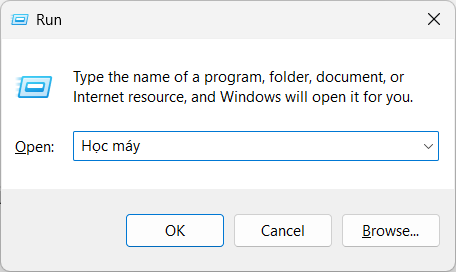
\includegraphics[width=8.84cm]{image1.png}
  \caption{Hộp thoại Run của Windows}
  \label{fig:run}
\end{figure}

Bước 2: Trong cửa sổ dòng lệnh (Hình~\ref{fig:cmd}), cài đặt thư viện và
chạy chương trình:

\begin{lstlisting}[language=bash,numbers=none]
pip install -r requirements.txt
streamlit run app.py
\end{lstlisting}

\begin{figure}[H]
  \centering
  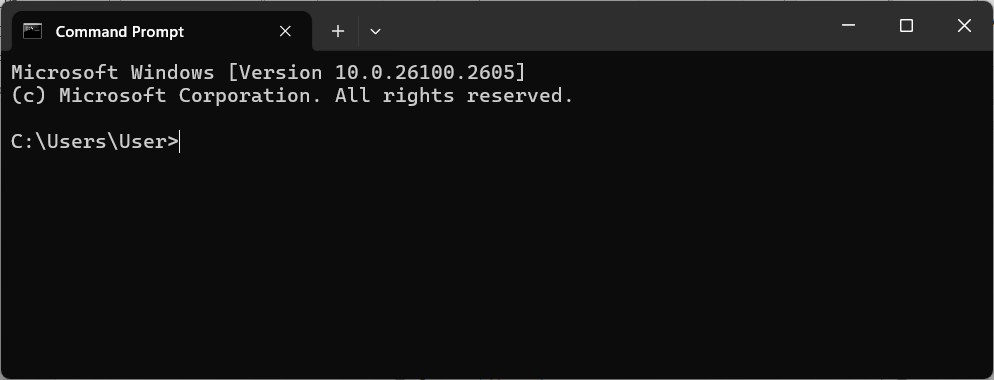
\includegraphics[width=11.12cm]{image2.png}
  \caption{Cửa sổ dòng lệnh CMD}
  \label{fig:cmd}
\end{figure}

Bước 3: Chương trình demo hiển thị trên trình duyệt (Hình~\ref{fig:chrome}).

\begin{figure}[H]
  \centering
  
\includegraphics[width=\textwidth]{image3.png}
  \caption{Giao diện chương trình demo trên trình duyệt Chrome}
  \label{fig:chrome}
\end{figure}

\chapter{Nhật ký đóng góp của các thành viên}
\label{pl:nhatky}

\begin{table}[H]
  \centering
  \caption{Nhật ký công việc theo tuần}
  \label{tab:nhatky}
  \begin{tabularx}{\textwidth}{>{\centering\arraybackslash}p{1.4cm} >{\centering\arraybackslash}p{2.4cm} p{3.2cm} X}
    \toprule
    \textbf{Tuần} & \textbf{Ngày} & \textbf{Thành viên} & \textbf{Công việc / commit} \\
    \midrule
    1 & \dots & \svAten & \dots \\
    1 & \dots & \svBten & \dots \\
    \dots & \dots & \dots & \dots \\
    \bottomrule
  \end{tabularx}
\end{table}

\end{document}
